\section{Introduction}
\label{hpca:sec:intro}

Contemporary server applications feature massive instruction footprints stemming from deeply layered software stacks. These footprints may far exceed the capacity of the branch target buffer (BTB) and instruction cache (L1-I), resulting in the so-called front-end bottleneck. BTB misses may lead to wrong-path execution, triggering a pipeline flush when misspeculation is detected. Such pipeline flushes not only throw away tens of cycles of work but also expose the fill latency of the pipeline. Similarly, L1-I misses cause the core front-end to stall for tens of cycles while the miss is being served from lower-level caches. 

BTB stands at the center of a high-performance core front end for three key reasons: it determines the instruction stream to be fetched, it identifies branches for the branch direction predictor, and it affects the L1-I hit rate. Specifically, by identifying control flow divergences, the BTB ensures that the branch direction predictor can make predictions for upcoming conditional branches. For predicted-taken and unconditional branches, the BTB supplies targets to which instruction fetch should be redirected. Finally, the BTB together with the direction predictor enables an important class of instruction prefetchers called fetch-directed instruction prefetchers (FDIP)~\cite{fdip, boomerang, shotgun, shotgunTOCS}, which rely on the BTB to discover L1-I prefetch candidates. 

Considering the criticality of capturing the large branch working sets of modern workloads, commercial CPUs feature BTBs with colossal capacities, a trend also observed by ~\cite{rebase}. With each BTB entry potentially requiring 8 bytes or more (\Cref{hpca:sec:background}), BTB storage costs can easily reach into tens and even hundreds of KBs. Indeed, the Samsung Exynos M6 mobile processor allocates a staggering 529KB of on-chip storage to BTBs~\cite{exynos}. Not only the BTB storage cost is high, it is increasing at a rapid pace. For example, the Samsung Exynos BTB storage budget increased nearly six fold (98.9KB to 561.5KB) from M2 to M6, over a period of about eight years~\cite{exynos}. While such massive BTBs are effective at capturing branch working sets, they do so at staggering area costs.

To reduce the BTB storage cost, prior work~\cite{DUPN, ittage, pdede} has focused on compressing the branch targets as they account for the majority of BTB storage budget as shown in \Cref{hpca:fig:conv-btb}. Concretely, Seznec~\cite{DUPN, ittage} observes that all branch targets within a page share the same page number and BTB storage requirements can be significantly reduced by storing the page number only once per page instead of once per target. To exploit this observation, he partitions the BTB in two structures, Main-BTB and Page-BTB, each storing different portions of branch targets. The Main-BTB stores the page offset and a pointer to the Page-BTB entry that stores the page number. The state-of-the-art BTB organization, PDede~\cite{pdede}, further observes that target addresses span significantly fewer \emph{regions} than pages, where a region is a group of contiguous pages. Therefore, it partitions the BTB even further and introduces a Region-BTB that lowers page number storage cost as the region number for all pages inside a region is stored only once. By storing page/region numbers only once for all branches in a page/region, these BTBs avoid information duplication, thus reducing storage requirements.

Though, these designs significantly reduce BTB storage requirements, they introduce several complexities that increase their access latency and power requirements. First, these designs introduce a level of indirection, i.e., on a BTB access, Main-BTB is accessed first to get the pointers to the Page-BTB and Region-BTB and only then these BTBs can be accessed. This sequential access, Main-BTB followed by Page/Region-BTBs, increases the overall BTB access latency which either requires a two-cycle BTB lookup or a longer clock period. Both of these alternatives incur a performance penalty. Second, on allocating a new BTB entry, Page-BTB and Region-BTB need to be searched to check if the page/region number for the target address is already present or not. As the page/region number can be anywhere in Page/Region-BTB, a fully-associative associative search is required~\cite{ittage} which increases BTB power requirements. An alternative is to restrict the locations where a page/region number can be stored in Page/Region-BTB~\cite{pdede}; however, it increase the likelihood of conflict misses.

This work seeks to reduce BTB storage requirements without increasing BTB complexity. To that end, we propose to store target offsets, defined as delta between the address of the branch instruction and that of its target, instead of full or compressed (i.e., page offset, page number, and region number) targets. Our key insight is that target offsets are unevenly distributed but tend to require significantly fewer bits to represent than full and even compressed target addresses. Our analysis reveals that 54\% of dynamic branches require only 6 bits or fewer for offset encoding, while a meager 1\% of branches need 25 bits or more to store their offsets.

\begin{figure}
\centering
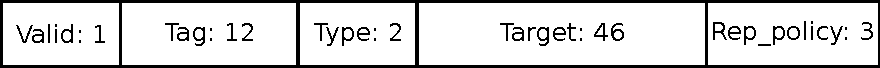
\includegraphics[width=\columnwidth]{figures/i_btb.pdf}
\caption {Composition of an entry in conventional BTB. The numbers are the number of bits required to encode each field.}
\label{hpca:fig:conv-btb}
\end{figure}

Based on this insight, we propose to store target offsets in the BTB rather than compressed or full target addresses, which can be up to 64 bits long depending on the size of virtual address space. To accommodate the varied distribution of target offsets, we size different ways of a set associative BTB to hold different number of offset bits such that each way stores only those branches whose target offsets can be encoded with a certain number of bits. In doing so, we not only significantly reduce BTB storage requirements but also avoid the complexities, indirection and fully-associative searches of the state-of-the-art BTB designs.
%We further observe that the tag field is the second-largest contributor to each BTB entry's storage requirement. To reduce this cost, we propose compressing the tags through the use of hashing.

This paper introduces BTB-X, a simple yet highly storage-effective BTB organization, that incarnates our idea of storing target offsets. BTB-X is a set associative BTB with its ways sized to store different sized target offsets. Our evaluation shows that BTB-X can track about 2.24x more branches than a conventional BTB storing full targets and about 1.3x more branches than PDede, a state-of-the-art BTB organization, with the same storage budget. Conversely, BTB-X can accommodate the same number of branches as conventional BTB and PDede while requiring 2.24x and 1.3x less storage. This work makes the following key contributions:

\begin{itemize}
    %\item We observe that the branch targets are the largest contributor to BTB storage cost, accounting for 42\% to 73\% of the storage cost in different BTB organization.
    \item We show that storing branch target offsets, instead of full or compressed target addresses, can provide drastic BTB storage savings because about 54\% of branches require only 6 bits or fewer to encode their offsets. A further 22\% of branches require between 7 and 10 bits. 
    \item We show that the target offset sizes are unevenly distributed with 0-6 bits, 7-10 bits, and 11-25 bits required to encode the offsets of 54\%, 22\% and 23\% of branches respectively. Therefore, a single size offset field cannot provide storage optimal solution.
    \item We introduce BTB-X, a simple and highly storage-effective BTB organization, that stores target offsets instead of targets themselves. Furthermore, BTB-X ways are sized to hold different sized target offsets.  
    \item We demonstrate that, with the same storage budget, BTB-X can accommodate about 2.24x and 1.3x more branches than a conventional BTB and PDede, a state-of-the-art BTB. Our evaluation further shows that BTB-X outperforms the conventional BTB even when provisioned with just half the storage budget.
\end{itemize}
